\chapter{Modellazione del sistema}
\label{modellazione}

In questo capitolo verranno inizialmente descritti gli attori che concorrono alle operazioni di registrazione/autenticazione per poi definire il flusso delle operazioni stesse.

\section{Attori}
\label{attori}

Lo schema di seguito rappresenta lo stato attuale dello standard FIDO in accordo all'implementazione descritta successivamente.
\begin{center}
	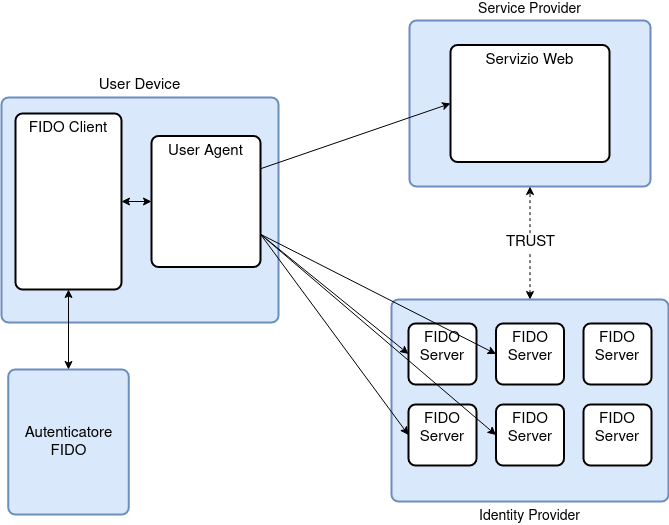
\includegraphics[width=.8\columnwidth]{figures/attori.png}
	\label{fig:attori}
\end{center}


Il protocollo include i seguenti attori: l'utente, Service Provider, Identity Provider, un numero \emph{n} di Identity Server, l'autenticatore hardware e il FIDO Client. 

Il \textbf{Service Provider} è un fornitore di un generico servizio a cui l'utente è interessato ad accedere. Può essere un qualunque servizio di streaming, banking, shopping etc. il quale fa uso di un intermediario per l'autenticazione dei propri utenti. Questo può avvenire per varie ragioni sia economiche che legate alla sicurezza. 
Il Service Provider definisce il \textbf{security level} per indicare il livello di \emph{survivability} desiderato, cioè il numero di Identity Server necessari a completare le operazioni di autenticazione/registrazione. Tale valore è un intero positivo e viene stabilito in funzione della confidenzialità del servizio erogato.

L'\textbf{Identity Provider} è un ente terzo che si occupa di fornire a un Service Provider il servizio di autenticazione. A tale scopo si avvale di \emph{n} Identity Server.
Compito dell'Identity Provider è anche quello di fornire il token di autenticazione al client da presentare al Service Provider per fare in modo che l'utente possa accedere al servizio scelto.
I vari Identity Server memorizzano le credenziali degli utenti ed una chiave segreta con cui autenticare token di autenticazione.

L'\textbf{autenticatore} hardware è un dispositivo che, tramite l'interazione con l'utente, permette l'accesso al servizio web richiesto. L'autenticatore si occupa di memorizzare le credenziali. Ogni credenziale contiene una chiave privata, metadati e un \textbf{array associativo} di contatori ${arr_C}$. L'${arr_C}$ associa ad un determinato \emph{security level} il valore di un \emph{contatore} intero per tenere traccia delle operazioni effettuate con successo. L'autenticatore ricorre alla chiave privata per firmare le challenge che gli sono sottoposte e invia la chiave pubblica al server così che esso possa verificare l'autenticità delle firme. 
Per la fase di creazione e le successive di autenticazione viene richiesto all'utente di compiere un'azione: essa può essere la pressione di un pulsante sulla chiavetta stessa, un collegamento NFC oppure ancora l'identificazione tramite impronta digitale. Così facendo l'operazione in corso viene autorizzata.

Il FIDO \textbf{Client} è un dispositivo che sfrutta un \textbf{User Agent} conforme ad implmentare le specifiche FIDO per il dialogo con l'Identity Server e con l'autenticatore, in collaborazione con l'hardware sottostante su cui è installato l'User Agent, tipicamente un sistema operativo. Il client è quindi interposto tra il FIDO Server e l'autenticatore fisico, agendo da intermediario. Il suo compito è duplice:
\begin{itemize}
	\item Comunicare con il server al fine di iniziare, e successivamente terminare, le operazioni di autenticazione e di creazione delle credenziali 
	\item Comunicare con l'autenticatore allo scopo di creare le chiavi crittografiche e firmare le challenge ricevute dal server
\end{itemize}
La comunicazione è bidirezionale e segue i protocolli definiti dagli standard: CTAP per l'interazione con l'autenticatore e WebAuthn per la comunicazione con il FIDO Server. 
Nel caso particolare dell'estensione survivable il client si occupa di replicare le operazioni su \emph{n} FIDO Server distinti, computando l'hash delle challenge ricevute e fornendolo all'autenticatore come un digest unico su cui apportare la firma. 


\section{Flusso operativo}
\label{flusso_operativo}

Il flusso operativo si compone di due operazioni distinte: una fase di creazione delle credenziali e una fase di autenticazione dell'utente. Tali operazioni vengono svolte, rispettivamente, durante la registrazione al servizio del Service Provider e a tutti le autenticazioni successive.

\subsection{Fase di registrazione}
\label{registrazione}

Alla fase di registrazione partecipano: l'utente, il FIDO Client, lo User Agent, \emph{n} Identity Server, l'autenticatore.

La fase di registrazione si origina a partire dalla richiesta dell'utente, utilizzando un User Agent, di registrarsi ad un servizio, offerto da un Service Provider, che supporti l'autenticazione passworldess, tramite degli Identity Provider. Il Service Provider fornisce all'utente il livello di sicurezza \emph{n} necessario per completare l'operazione. La fase di creazione dovrà essere replicata dal client su tutti gli \emph{n} Identity Server presenti.  Il processo messo in atto è il seguente:

\begin{enumerate}
	\item Ogni Identity Server crea il proprio stato interno e la challenge
	\item Ogni Identity Server invia al Client una serie di requisiti secondo cui deve essere svolta la cerimonia di registrazione, e la challenge generata
	\item Il Client salva tutte le challenge ricevute in un vettore e computa l'hash dello stesso
	\item Il Client effettua una chiamata al metodo opportuno dell'autenticatore, fornendo i requisiti di creazione richiesti dall'Identity Server e il digest computato come challenge
	\item L'autenticatore procede a generare la coppia di chiavi crittografiche seguendo le imposizioni del server e invia al client la challenge firmata accompagnata dalla chiave pubblica e il contatore specifico dell'${arr_C}$ inizializzato a uno.
	\item Il Client invia ad ogni Identity Server il vettore con le challenge, l'hash dello stesso, la firma, la chiave pubblica e il signature counter ricevuto
	\item Ogni Identity Server controlla che la challenge da lui generata sia presente all'interno del vettore e controlla, computando lui stesso l'hash del vettore, l'integrità di quanto ricevuto. Infine, verifica tramite la chiave pubblica fornitagli l'autenticità della firma.
	\item Qualora il processo sia andato a buon fine, gli Identity Server salveranno le informazioni ricevute (contatore, chiave pubblica, identificatore del client) al proprio interno
\end{enumerate} 

\subsection{Fase di autenticazione}
\label{autenticazione}

La fase di autenticazione ricalca i passaggi di quella di registrazione con la differenza che gli Identity Server sono già in possesso della chiave pubblica con cui verificare l'autenticità della firma apportata alle challenge. 

In questa fase viene comunicato un security level pari a ${|Q|}$ da parte del Service Provider, cioè la cardinalità del sottoinsieme di Identity Server con cardinalità $Q:$ ${|Q|\leq n}$ presso cui è necessario autenticarsi. Questo valore prende in considerazione la tollerabilità alle intrusione che ha il Service Provider. In particolare: ${|Q| \in [(2k+1), (3k+1)] }$, dove \emph{k} rappresenta il numero di Identity Server di cui si può tollerare la compromissione. 

\begin{enumerate}
	\item Ogni Identity Server crea il proprio stato interno e la challenge
	\item Ogni Identity Server invia al Client una serie di requisiti, secondo cui deve essere svolta la cerimonia di autenticazione, e la challenge generata
	\item Il Client salva tutte le challenge ricevute in un vettore e computa l'hash dello stesso
	\item Il Client effettua una chiamata al metodo opportuno dell'autenticatore, fornendo i requisiti di autenticazione richiesti dall'Identity Server e il digest computato come challenge
	\item L'autenticatore incrementa il contatore dell'${arr_C}$ specifico. Invia poi al Client la challenge firmata e il contatore aggiornato
	\item Il Client invia ad ogni Identity Server il vettore con le challenge, l'hash dello stesso, la firma ricevuta e il signature counter
	\item Ogni Identity Server controlla che la challenge da lui generata sia presente all'interno del vettore e controlla, computando lui stesso l'hash del vettore, l'integrità di quanto ricevuto. Infine, verifica tramite la chiave pubblica, memorizzata precedentemente, l'autenticità della firma
	\item Ogni Identiy Server controlla che il \emph{signature counter} ricevuto sia maggiore di quello memorizzato in precedenza e in tal caso aggiorna quest'ultimo con il valore appena ricevuto
	\item Se i passaggi precedenti sono avvenuti con successo rilasciano al Client il token di autenticazione tramite cui può completare l'autenticazione presso il Service Provider
\end{enumerate}